\documentclass[aps,pra,reprint]{revtex4-2}
\usepackage[table,xcdraw]{xcolor}
\usepackage{amsmath,amsthm,amssymb, color}
\usepackage[colorlinks,hypertexnames=false]{hyperref}
\usepackage{color}
\usepackage{tikz}
\usetikzlibrary{positioning}
\usetikzlibrary{quotes}

\begin{document}

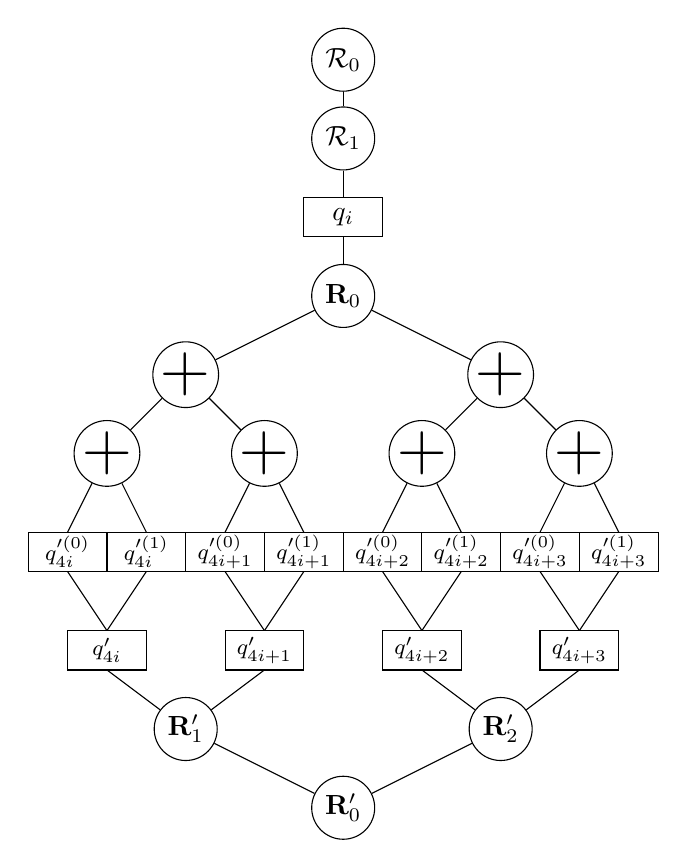
\begin{tikzpicture}
% Linear routers
\node[draw, circle,minimum size=0.8cm,inner sep=0pt] (l0) at (3,5){$\mathcal{R}_0$};
\node[draw, circle,minimum size=0.8cm,inner sep=0pt] (l1) at (3,4){$\mathcal{R}_1$};
\draw (2.5, 2.75)  rectangle node{$q_{i}$} ++(1,0.5);
\draw[] (l0) to (l1);
\draw[] (l1) to (3,3.25);

% top half
\node[draw, circle,minimum size=0.8cm,inner sep=0pt] (t0) at (3,2){$\mathbf{R}_0$};
\node[draw, circle,minimum size=0.8cm,inner sep=0pt] (t1) at (1,1){\Huge +};
\node[draw, circle,minimum size=0.8cm,inner sep=0pt] (t2) at (5,1){\Huge +};
\draw[] (t0) to (t1);
\draw[] (t0) to (t2);
\draw[] (3,2.75) to (t0);

\node[draw, circle,minimum size=0.8cm,inner sep=0pt] (x0) at (0,0){\Huge +};
% 
\node[draw, circle,minimum size=0.8cm,inner sep=0pt] (x1) at (2,0){\Huge +};
% 
\node[draw, circle,minimum size=0.8cm,inner sep=0pt] (x2) at (4,0){\Huge +};
% 
\node[draw, circle,minimum size=0.8cm,inner sep=0pt] (x3) at (6,0){\Huge +};
% 
\draw[] (x0) to (t1);
\draw[] (x1) to (t1);
\draw[] (x2) to (t2);
\draw[] (x3) to (t2);
% Bottom half
\draw (-1, -1.5)  rectangle node{\footnotesize $q'^{(0)}_{4i}$} ++(1,0.5);
\draw (0, -1.5)  rectangle node{\footnotesize$q'^{(1)}_{4i}$} ++(1,0.5);
\draw (1, -1.5)  rectangle node{\footnotesize$q'^{(0)}_{4i+1}$} ++(1,0.5);
\draw (2, -1.5)  rectangle node{\footnotesize$q'^{(1)}_{4i+1}$} ++(1,0.5);
\draw (3, -1.5)  rectangle node{\footnotesize$q'^{(0)}_{4i+2}$} ++(1,0.5);
\draw (4, -1.5)  rectangle node{\footnotesize$q'^{(1)}_{4i+2}$} ++(1,0.5);
\draw (5, -1.5)  rectangle node{\footnotesize$q'^{(0)}_{4i+3}$} ++(1,0.5);
\draw (6, -1.5)  rectangle node{\footnotesize$q'^{(1)}_{4i+3}$} ++(1,0.5);

\draw[] (x0) to (-0.5,-1);
\draw[] (x0) to (0.5,-1);
\draw[] (x1) to (1.5,-1);
\draw[] (x1) to (2.5,-1);
\draw[] (x2) to (3.5,-1);
\draw[] (x2) to (4.5,-1);
\draw[] (x3) to (5.5,-1);
\draw[] (x3) to (6.5,-1);

\node[draw, circle,minimum size=0.8cm,inner sep=0pt] (t1p) at (1,-3.5){$\mathbf{R}'_1$};
\node[draw, circle,minimum size=0.8cm,inner sep=0pt] (t2p) at (5,-3.5){$\mathbf{R}'_2$};
\node[draw, circle,minimum size=0.8cm,inner sep=0pt] (t0p) at (3,-4.5){$\mathbf{R}'_0$};

% 
\draw (-.5, -2.75)  rectangle node{\footnotesize $q'_{4i}$} ++(1,0.5);
% 
\draw (1.5, -2.75)  rectangle node{\footnotesize $q'_{4i+1}$} ++(1,0.5);
% 
\draw (3.5, -2.75)  rectangle node{\footnotesize $q'_{4i+2}$} ++(1,0.5);
% 
\draw (5.5, -2.75)  rectangle node{\footnotesize $q'_{4i+3}$} ++(1,0.5);


\draw[] (0,-2.25) to (-0.5,-1.5);
\draw[] (0,-2.25) to (0.5,-1.5);
\draw[] (2,-2.25) to (1.5,-1.5);
\draw[] (2,-2.25) to (2.5,-1.5);
\draw[] (4,-2.25) to (3.5,-1.5);
\draw[] (4,-2.25) to (4.5,-1.5);
\draw[] (6,-2.25) to (5.5,-1.5);
\draw[] (6,-2.25) to (6.5,-1.5);

\draw[] (t1p) to (0,-2.75);
\draw[] (t1p) to (2,-2.75);
\draw[] (t2p) to (4,-2.75);
\draw[] (t2p) to (6,-2.75);
\draw[] (t0p) to (t1p);
\draw[] (t0p) to (t2p);

\end{tikzpicture}

\end{document}